%% LyX 2.3.6.1 created this file.  For more info, see http://www.lyx.org/.
%% Do not edit unless you really know what you are doing.
\documentclass[english]{article}
\usepackage[T1]{fontenc}
\usepackage[latin9]{inputenc}
\usepackage{geometry}
\geometry{verbose,tmargin=2.5cm,bmargin=2.5cm,lmargin=2.5cm,rmargin=2.5cm}
\usepackage{array}
\usepackage{calc}
\usepackage{textcomp}
\usepackage{graphicx}

\makeatletter

%%%%%%%%%%%%%%%%%%%%%%%%%%%%%% LyX specific LaTeX commands.
%% Because html converters don't know tabularnewline
\providecommand{\tabularnewline}{\\}

\makeatother

\usepackage{babel}
\begin{document}
{[}SPLIT\_HERE{]}
\begin{enumerate}
\item \textbf{{[}ALVL/9597/2019/P1/Q1{]} }

Many applications require the user to search for a data item from
a file or one-dimensional array.

\texttt{JARGON.TXT} is a text file containing computing terms with
one term per line. The program will read all the terms from \texttt{JARGON.TXT}
into an array.

The user will choose if the type of search is to find:
\begin{enumerate}
\item[1.]  An exact match 
\item[2.]  A match at the beginning of the term text
\item[3.]  A match anywhere within the term text
\end{enumerate}

\subsubsection*{Task 1.1}

Design and write program code to:
\begin{itemize}
\item Read the entire contents of \texttt{JARGON.TXT} into an array 
\item Allow the user to repeatedly select the type of search, then input
a term 
\item Output the matching term(s) found 
\item Output a count of the number of matches 
\item End with the input of term \textquotedbl XXX\textquotedbl{}
\end{itemize}
A typical run of the program is shown below:

\texttt{+++++++++++++++++++++++ }

\texttt{1. Exact match }

\texttt{2. Start of term }

\texttt{3. Within term }

\texttt{++++++++++++++++++ }

\texttt{Choice ?1 }

\texttt{Term?firewall }

\texttt{firewall }

\texttt{There were 1 matching term(s)}

\texttt{+++++++++++++++++++++++ }

\texttt{1. Exact match }

\texttt{2. Start of term }

\texttt{3. Within term }

\texttt{++++++++++++++++++ }

\texttt{Choice ?2 }

\texttt{Term?data }

\texttt{data flow diagram }

\texttt{database management system }

\texttt{data file }

\texttt{database }

\texttt{There were 4 matching term(s)}

\texttt{+++++++++++++++++++++++ }

\texttt{1. Exact match }

\texttt{2. Start of term }

\texttt{3. Within term }

\texttt{++++++++++++++++++}

\texttt{Choice ?3 }

\texttt{Term?box }

\texttt{white box testing }

\texttt{black box testing }

\texttt{There were 2 matching term(s)}

\subsubsection*{Evidence 1}

The program code. \hfill{}{[}11{]}

\subsubsection*{Task 1.2}

Study the contents of \texttt{JARGON.TXT} and then design four test
cases to thoroughly test the working of your program code.

\subsubsection*{Evidence 2}

State the test data used in Task 1.2 and show screenshots to confirm
the successful testing of each of your four test cases. \hfill{}{[}4{]}

{[}SPLIT\_HERE{]}
\item \textbf{{[}ALVL/9597/2019/P1/Q2{]} }

A binary search (binary chop) is a technique to search for a value
in an ordered dataset.

\subsubsection*{Task 2.1}

Study the identifier table and incomplete recursive algorithm. 

The missing parts of the algorithm are labelled A, B and C.
\begin{center}
\begin{tabular}{|l|c|l|}
\hline 
\texttt{\hspace{0.01\columnwidth}}Variable & \texttt{\hspace{0.01\columnwidth}}Data Type & \texttt{\hspace{0.05\columnwidth}}Description\tabularnewline
\hline 
\texttt{ThisArray} & \texttt{ARRAY OF STRING} & Array containing the the dataset\tabularnewline
\hline 
\texttt{FindValue} & \texttt{STRING} & Item to be found\tabularnewline
\hline 
\texttt{Low} & \texttt{INTEGER} & Lowest index of the considered list\tabularnewline
\hline 
\texttt{High} & \texttt{INTEGER} & Highest index of the considered list\tabularnewline
\hline 
\texttt{Middle} & \texttt{INTEGER} & The array index for the middle position of the current list considered\tabularnewline
\hline 
\end{tabular}
\par\end{center}

\noindent %
\noindent\begin{minipage}[t]{1\columnwidth}%
\texttt{FUNCTION BinarySearch(ThisArray, FindValue, Low, High) RETURNS
INTEGER}

\texttt{\qquad{}DECLARE Middle : INTEGER}

\texttt{\qquad{}IF ............... A ...............}

\texttt{\qquad{}\qquad{}THEN}

\texttt{\qquad{}\qquad{}\qquad{}RETURN -1 // not found}

\texttt{\qquad{}ELSE}

\texttt{\qquad{}\qquad{}// calculate new Middle value}

\texttt{\qquad{}\qquad{}Middle \textleftarrow{} ............... B
...............}

\texttt{\qquad{}\qquad{}IF ThisArray{[}Middle{]} > FindValue}

\texttt{\qquad{}\qquad{}\qquad{}THEN}

\texttt{\qquad{}\qquad{}\qquad{}\qquad{}RETURN BinarySearch(ThisArray,
FindValue, Low, Middle - 1)}

\texttt{\qquad{}\qquad{}\qquad{}ELSE}

\texttt{\qquad{}\qquad{}\qquad{}\qquad{}IF ThisArray{[}Middle{]}
< FindValue}

\texttt{\qquad{}\qquad{}\qquad{}\qquad{}\qquad{}THEN}

\texttt{\qquad{}\qquad{}\qquad{}\qquad{}\qquad{}\qquad{}............... C
...............}

\texttt{\qquad{}\qquad{}\qquad{}\qquad{}\qquad{}ELSE}

\texttt{\qquad{}\qquad{}\qquad{}\qquad{}\qquad{}\qquad{}RETURN
Middle // found at position Middle}

\texttt{\qquad{}\qquad{}\qquad{}\qquad{}ENDIF}

\texttt{\qquad{}\qquad{}ENDIF}

\texttt{\qquad{}ENDIF}

\texttt{ENDFUNCTION}%
\end{minipage}

\subsubsection*{Evidence 3}

What are the three missing lines in this pseudocode? \hfill{}{[}3{]}

\subsubsection*{Task 2.2}

Write a program to implement binary search. 

The program will
\begin{itemize}
\item Call procedure InitialiseAnimals 
\item Input an animal name
\item Use the function BinarySearch 
\item Report whether or now this animal name was found. If found, also output
the index position.
\end{itemize}
The array in the program has identifier \texttt{MyAnimal}. 

Use the dataset given in the file \texttt{ANIMALS.TXT}. You should
paste the contents of this file into your program. The statements
will form the basis of the code for the procedure \texttt{InitialiseAnimals}.

\subsubsection*{Evidence 4}

Program code for Task 2.2 \hfill{}{[}7{]}

\subsubsection*{Evidence 5}

Screenshot to confirm that an animal wich is present in the list was
found with its index position displayed. \hfill{}{[}1{]}

\subsubsection*{Task 2.3}

Amend the program as follows: 

The program must also output the number of function calls carried
out.

\subsubsection*{Evidence 6}

The amended program code. \hfill{}{[}4{]}

\subsubsection*{Evidence 7}

Screenshots showing the amended ouput for runs of the program where: 
\begin{itemize}
\item the animal is found
\item the animal is not found. \hfill{}{[}2{]}
\end{itemize}
{[}SPLIT\_HERE{]}
\item \textbf{{[}ALVL/9597/2019/P1/Q3{]} }

A program is to be written to represent and implement a linked list
of nodes. Each node contains a string data value and a pointer. The
pointers link the data items in alphabetical order. 

The unused nodes are linked as shown below. The first unused node
is the position where the next new data item is to be stored. 
\begin{center}
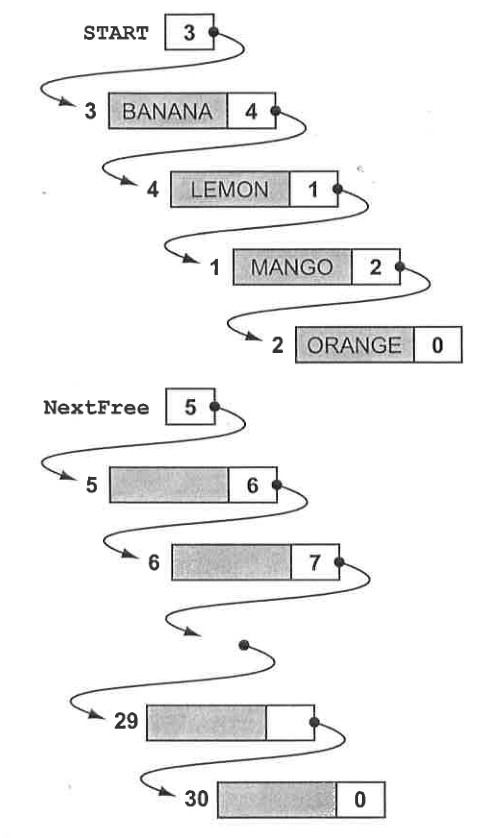
\includegraphics[width=0.25\paperwidth]{C:/Users/Admin/Desktop/Github/question_bank/LyX/static/img/9597-ALVL-2014-P1-Q3}
\par\end{center}

The diagram shows the linked list with: 
\begin{itemize}
\item the items MANGO, ORANGE, BANANA and LEMON (added in that order). 
\item the unused nodes linked together.
\end{itemize}
Each node is implemented as an instance of the class\texttt{ ListNode}.
The class \texttt{ListNode} has the following properties: 
\begin{center}
\begin{tabular}{|l|c|l|}
\hline 
\multicolumn{3}{|c|}{Class\texttt{: ListNode}}\tabularnewline
\hline 
\multicolumn{3}{|c|}{Properties}\tabularnewline
\hline 
\texttt{\hspace{0.01\columnwidth}}Identifier & \texttt{\hspace{0.01\columnwidth}}Data Type & \texttt{\hspace{0.01\columnwidth}}Description\tabularnewline
\hline 
\texttt{DataValue} & \texttt{STRING} & The node data\tabularnewline
\hline 
\texttt{PointerValue} & \texttt{INTEGER} & The node pointer\tabularnewline
\hline 
\end{tabular}
\par\end{center}

A linked list is implemented as an instance of the class \texttt{LinkedList}.
The class \texttt{LinkedList} has the following properties and methods: 
\begin{center}
\begin{tabular}{|l|c|>{\raggedright}p{0.25\columnwidth}|}
\hline 
\multicolumn{3}{|c|}{Class\texttt{: LinkedList}}\tabularnewline
\hline 
\multicolumn{3}{|c|}{Properties}\tabularnewline
\hline 
\texttt{\hspace{0.01\columnwidth}}Identifier & \texttt{\hspace{0.01\columnwidth}}Data Type & \texttt{\hspace{0.01\columnwidth}}Description\tabularnewline
\hline 
\texttt{Node} & \texttt{ARRAY{[}30{]} OF ListNode} & The linked list data structure --- data values and pointers.The array
index starts at 1.For testing purposes the dataset has a maximum of
30 items.\tabularnewline
\hline 
\texttt{Start} & \texttt{INTEGER} & Index position of the node at the start of the linked list\tabularnewline
\hline 
\texttt{NextFree} & \texttt{INTEGER} & Index position of the next unused node \tabularnewline
\hline 
\multicolumn{3}{|l|}{Methods}\tabularnewline
\hline 
\texttt{\hspace{0.01\columnwidth}}Identifier &  & \texttt{\hspace{0.01\columnwidth}}Description\tabularnewline
\hline 
\texttt{Initialise} & \texttt{PROCEDURE} & Sets all the node data values to \textquoteleft empty string\textquoteright .

Set pointers to indicate all nodes are unused and linked.

lnitialise values for \texttt{Start} and \texttt{NextFree}.\tabularnewline
\hline 
\texttt{AddNode} & \texttt{PROCEDURE} & Add a new data item to the linked list.\tabularnewline
\hline 
\texttt{Traversal} & \texttt{PROCEDURE} & Display the data items in order.\tabularnewline
\hline 
\texttt{ReverseTraversal} & \texttt{PROCEDURE} & Display the data items in reverse order.\tabularnewline
\hline 
\texttt{DisplayLinkedList} & \texttt{PROCEDURE} & Display the current state of pointers and the array contents.\tabularnewline
\hline 
\texttt{IsEmpty} & \texttt{FUNCTION RETURNS BOOLEAN} & Tests for empty linked list.\tabularnewline
\hline 
\texttt{IsFull} & \texttt{FUNCTION RETURNS BOOLEAN} & Tests for no unused nodes.\tabularnewline
\hline 
\end{tabular}
\par\end{center}

\subsubsection*{Task 3.1}

Write program code that repeatedly:
\begin{itemize}
\item displays a menu with the following choices: 
\begin{enumerate}
\item[1.]  Add an item 
\item[2.]  Traverse the linked list of used nodes and output the data values 
\item[3.]  Output all pointers and data values 
\item[4.]  Exit 
\end{enumerate}
\item calls an appropriate procedure depending on the user's choice. 
\end{itemize}

\subsubsection*{Evidence 8}

Program code for Task 3.1.\hfill{} {[}5{]}

\subsubsection*{Task 3.2}

Write program code for the classes \texttt{ListNode} and \texttt{LinkedList}
including the \texttt{IsEmpty} method. The code should follow the
specification given. 

Do not attempt to write the methods \texttt{AddNode}, \texttt{Traversal},
\texttt{ReverseTraversal} or \texttt{IsFull} at this stage. 

\subsubsection*{Evidence 9}

Program code for the \texttt{ListNode} and \texttt{LinkedList} classes
(Task 3.2).\hfill{} {[}12{]}

\subsubsection*{Task 3.3}

Write code to create a \texttt{LinkedList} object in the main program.

Run the program and select menu choice 3 to confirm the initial values
of the pointers and data values when the linked list is empty. {[}10{]}

\subsubsection*{Evidence 10}

Screenshot confirming all values after initialisation of the \texttt{LinkedList}
object (Task 3.3). 

\hfill{} {[}3{]}

\subsubsection*{Task 3.4}

Consider the \texttt{AddNode} method. The following algorithm will
add a new data item to the linked list. 

The algorithm uses the variables below:
\begin{center}
\begin{tabular}{|l|c|>{\raggedright}p{0.25\columnwidth}|}
\hline 
\texttt{\hspace{0.01\columnwidth}}Identifier & \texttt{\hspace{0.01\columnwidth}}Data Type & \texttt{\hspace{0.01\columnwidth}}Description\tabularnewline
\hline 
\texttt{NewItem} & \texttt{STRING} & New data item input by the user\tabularnewline
\hline 
\texttt{Found} & \texttt{BOOLEAN} & Flags to \texttt{TRUE} when the position at which to insert the new
item has been found\tabularnewline
\hline 
\texttt{Current} & \texttt{INTEGER} & Current array index position during list traversal\tabularnewline
\hline 
\texttt{Previous} & \texttt{INTEGER} & Previous array index position during list traversal\tabularnewline
\hline 
\texttt{Temp} & \texttt{INTEGER} & Temporary storage of pointer value\tabularnewline
\hline 
\end{tabular}
\par\end{center}

\noindent\fbox{\begin{minipage}[t]{1\columnwidth - 2\fboxsep - 2\fboxrule}%
\texttt{PROCEDURE AddNode }

\texttt{\qquad{}INPUT NewItem }

\texttt{\qquad{}Node{[}NextFree{]}.DataValue <\textemdash{} NewItem }

\texttt{\qquad{}IF Start = 0 }

\texttt{\qquad{}\qquad{}THEN }

\texttt{\qquad{}\qquad{}Start <\textemdash{} NextFree }

\texttt{\qquad{}\qquad{}Temp <\textemdash{} Node{[}NextFree{]}.PointerValue }

\texttt{\qquad{}\qquad{}Node{[}NextFree{]}.PointerValue <\textemdash{}
0 }

\texttt{\qquad{}\qquad{}NextFree <\textemdash{} Temp }

\texttt{\qquad{}ELSE }

\texttt{\qquad{}\qquad{}// traverse the list - starting at Start
to find }

\texttt{\qquad{}\qquad{}// the position at which to insert the new
item }

\texttt{\qquad{}\qquad{}Temp <\textemdash{} Node{[}NextFree{]}.PointerValue }

\texttt{\qquad{}\qquad{}IF NewItem < Node{[}Start{]}.DataValue }

\texttt{\qquad{}\qquad{}\qquad{}THEN }

\texttt{\qquad{}\qquad{}\qquad{}\qquad{}// new item will become
the start of the list }

\texttt{\qquad{}\qquad{}\qquad{}\qquad{}Node{[}NextFree{]}.PointerValue
<\textemdash{} Start }

\texttt{\qquad{}\qquad{}\qquad{}\qquad{}Start <\textemdash{} NextFree }

\texttt{\qquad{}\qquad{}\qquad{}\qquad{}NextFree <\textemdash{}
Temp }

\texttt{\qquad{}\qquad{}\qquad{}ELSE }

\texttt{\qquad{}\qquad{}\qquad{}\qquad{}// the new item is not
at the start of the list }

\texttt{\qquad{}\qquad{}\qquad{}\qquad{}Previous <\textemdash{}
0 }

\texttt{\qquad{}\qquad{}\qquad{}\qquad{}Current <\textemdash{}
Start }

\texttt{\qquad{}\qquad{}\qquad{}\qquad{}Found <\textemdash{} False }

\texttt{\qquad{}\qquad{}\qquad{}\qquad{}REPEAT }

\texttt{\qquad{}\qquad{}\qquad{}\qquad{}\qquad{}IF NewItem <=
Node{[}Current{]}.DataValue }

\texttt{\qquad{}\qquad{}\qquad{}\qquad{}\qquad{}\qquad{}THEN }

\texttt{\qquad{}\qquad{}\qquad{}\qquad{}\qquad{}\qquad{}\qquad{}Node{[}Previous{]}.PointerValue
<\textemdash{} NextFree }

\texttt{\qquad{}\qquad{}\qquad{}\qquad{}\qquad{}\qquad{}\qquad{}Node{[}NextFree{]}.PointerValue
<\textemdash{} Current }

\texttt{\qquad{}\qquad{}\qquad{}\qquad{}\qquad{}\qquad{}\qquad{}NextFree
<\textemdash{} Temp }

\texttt{\qquad{}\qquad{}\qquad{}\qquad{}\qquad{}\qquad{}\qquad{}Found
<\textemdash{} True }

\texttt{\qquad{}\qquad{}\qquad{}\qquad{}\qquad{}\qquad{}ELSE }

\texttt{\qquad{}\qquad{}\qquad{}\qquad{}\qquad{}\qquad{}\qquad{}//
move on to the next node }

\texttt{\qquad{}\qquad{}\qquad{}\qquad{}\qquad{}\qquad{}\qquad{}Previous
<\textemdash{} Current }

\texttt{\qquad{}\qquad{}\qquad{}\qquad{}\qquad{}\qquad{}\qquad{}Current
<\textemdash{} Node{[}Current{]}.PointerValue }

\texttt{\qquad{}\qquad{}\qquad{}\qquad{}\qquad{}ENDIF }

\texttt{\qquad{}\qquad{}\qquad{}\qquad{}UNTIL Found = True OR
Current = 0 }

\texttt{\qquad{}\qquad{}\qquad{}\qquad{}IF Current <\textemdash{}
0 }

\texttt{\qquad{}\qquad{}\qquad{}\qquad{}\qquad{}THEN }

\texttt{\qquad{}\qquad{}\qquad{}\qquad{}\qquad{}\qquad{}Node{[}Previous{]}.PointerValue
<\textemdash{} NextFree }

\texttt{\qquad{}\qquad{}\qquad{}\qquad{}\qquad{}\qquad{}Node{[}NextFree{]}.PointerValue
<\textemdash{} 0 }

\texttt{\qquad{}\qquad{}\qquad{}\qquad{}\qquad{}\qquad{}NextFree
<\textemdash{} Temp }

\texttt{\qquad{}\qquad{}\qquad{}\qquad{}ENDIF }

\texttt{\qquad{}\qquad{}ENDIF }

\texttt{\qquad{}ENDIF }

\texttt{ENDPROCEDURE }

Note: The above pseudocode is available in the text file \texttt{PSEUDOCODE\_TASK\_3\_4.TXT}%
\end{minipage}}

Write code to implement for the \texttt{LinkedList} class: 
\begin{itemize}
\item the \texttt{AddNode} method 
\item the \texttt{IsFull} method. 
\end{itemize}
You may use the text file \texttt{PSEUDOCODE\_TASK\_3\_4.TXT} as a
basis for the writing of your code. 

The main program should check each time that the \texttt{LinkedList}
object is not full before using the \texttt{AddNode} method. 

Run the program as follows: 
\begin{itemize}
\item Menu choice 1 four times, inputting the data values: 

MANGO, ORANGE. BANANA. LEMON in that order. 
\item Menu choice 3 to display. 
\end{itemize}

\subsubsection*{Evidence 11}

Program code for method \texttt{AddNode}. \hfill{}{[}8{]}

\subsubsection*{Evidence 12}

Screenshot showing the pointers and the addition of the four nodes
to the linked list.\hfill{} {[}3{]}

\subsubsection*{Task 3.5}

Write program code to implement the \texttt{LinkedList} class method
\texttt{Traversal} by calling the \texttt{TraversalInOrder} procedure
given below. 

\noindent %
\noindent\begin{minipage}[t]{1\columnwidth}%
\texttt{PROCEDURE TraversalInOrder(Index)}

\texttt{\qquad{}IF Index <> 0}

\texttt{\qquad{}\qquad{}THEN}

\texttt{\qquad{}\qquad{}\qquad{}OUTPUT Node{[}lndex{]}.DataValue}

\texttt{\qquad{}\qquad{}\qquad{}// follow the pointer to the next
data item in the linked list}

\texttt{\qquad{}\qquad{}\qquad{}TraversalInOrder(Node{[}Index{]}.PointerValue)}

\texttt{\qquad{}ENDIF}

\texttt{ENDPRCCEDURE}%
\end{minipage}

\subsubsection*{Evidence 13}

Program code for procedures \texttt{Traversal} and \texttt{TraversalInOrder}.\hfill{}
{[}2{]}

\subsubsection*{Task 3.6}

Run the program as follows: 
\begin{itemize}
\item Menu choice 1 four times, inputting the data values: 

MANGO, ORANGE, BANANA. LEMON in that order. 
\item Menu choice 2 to display. 
\end{itemize}

\subsubsection*{Evidence 14}

Screenshot showing the program execution to test the \texttt{Traversal}
method. \hfill{}{[}2{]}

\subsubsection*{Task 3.7}

Make a copy of the \texttt{TraversalInOrder} and \texttt{Traversal}
procedures.

Paste to form two new procedures \texttt{TraversalInReverseOrder}
and \texttt{ReverseTraversal}. 

Make the necessary changes/additions to these procedures in order
that the data items are output in reverse order by calling the new
method \texttt{ReverseTraversal}.

Run the program code from a new menu choice 4.

Test the method using the four items given in Task 3.6.

\subsubsection*{Evidence 15}

Program code for the new procedures. \hfill{}{[}2{]}

\subsubsection*{Evidence 16}

Screenshot showing option 4 selected and the resulting output. \hfill{}{[}1{]}

{[}SPLIT\_HERE{]}
\item \textbf{{[}ALVL/9597/2019/P1/Q4{]} }

Design and code a computer program to simulate the following: 

A garden has a rectangular fish pond measuring 15 metres by 8 metres. 

The pond is to be represented on the screen by a rectangular grid.
Each square metre of the pond is represented by an x-coordinate and
a y-coordinate. The top left square metre of the pond display has
x = 1 and y = 1. 

A boy throws a stone into the pond. The user will input the x-coordinate
and y-coordlnate of the stone impact position. 

A grid representing the pond is then displayed with the stone's impact
position: 

\texttt{X coordinate <1 to 15>? 9 }

\texttt{Y coordinate <1 to 8>? 3 }

\texttt{. . . . . . . . . . . . . . . }

\texttt{. . . . . . . . . . . . . . .}

\texttt{. . . . . . . . S . . . . . .}

\texttt{. . . . . . . . . . . . . . .}

\texttt{. . . . . . . . . . . . . . .}

\texttt{. . . . . . . . . . . . . . .}

\texttt{. . . . . . . . . . . . . . .}

\texttt{. . . . . . . . . . . . . . .}

\subsubsection*{Task 4.1}

The following are the suggested characters to use for the visual representation
of the pond: 
\begin{center}
\begin{tabular}{|c|c|l|}
\hline 
Character & ASCII code (decimal) & \texttt{\hspace{0.01\columnwidth}}Represents\tabularnewline
\hline 
. & 46 & One square metre of water\tabularnewline
\hline 
S & 83 & Stone impact position\tabularnewline
\hline 
\end{tabular}
\par\end{center}

Decide on the design to be used for: 
\begin{itemize}
\item The data structure to represent the grid
\item The contents of each square metre of the pond 
\item Procedure(s) and/or function(s)s to be used 
\end{itemize}

\subsubsection*{Evidence 17}

Show your program design (Task 4.1). \hfill{} {[}6{]}

\subsubsection*{Task 4.2}

Write program code to display the pond contents after a single stone
has been thrown. 

\subsubsection*{Evidence 18}

The program code. \hfill{} {[}7{]}

\subsubsection*{Evidence 19}

Screenshot for a single run of the program. \hfill{} {[}1{]}

\subsubsection*{Task 4.3}

The boy has been told to stop throwing stones into the pond because
the pond now has three fish. The fish randomly swim around. Each fish
will occupy a unique grid position.

Using a random number generator, simulate the positioning of the three
fish. 

Use the following character for a fish: 
\begin{center}
\begin{tabular}{|c|c|l|}
\hline 
Character & ASCII code (decimal) & \texttt{\hspace{0.01\columnwidth}}Represents\tabularnewline
\hline 
F & 70 & Fish\tabularnewline
\hline 
\end{tabular}
\par\end{center}

Write program code to show the pond containing the three fish at a
particular instance of time. The program will now only display the
pond and fish. 

\subsubsection*{Evidence 20}

The program code for Task 4.3. \hfill{} {[}6{]}

\subsubsection*{Evidence 21}

Screenshot for a single run of the program. \hfill{} {[}1{]}

\subsubsection*{Task 4.4}

The boy has been asked to feed the fish. He cannot see the fish in
the pond. He throws a food pellet into the pond which lands inside
one of the square metres. If one of the fish is in this square. it
eats the food and becomes a happy fish. 

Use character symbols for the pond\textquoteleft s grid display as
follows: 
\begin{center}
\begin{tabular}{|c|c|l|}
\hline 
Character & ASCII code (decimal) & \texttt{\hspace{0.01\columnwidth}}Represents\tabularnewline
\hline 
. & 46 & One square metre of water\tabularnewline
\hline 
P & 80 & Pellet (if not eaten by one of the fish)\tabularnewline
\hline 
H & 72 & Happy (fed) fish\tabularnewline
\hline 
F & 70 & Fish\tabularnewline
\hline 
\end{tabular}
\par\end{center}

Write program code to simulate the boy throwing one food pellet into
the pond. The user will input an x-coordinate and y-coordinate for
the food pellet position. You should consider the possible reuse of
any code from Tasks 4.2 and 4.3.

\subsubsection*{Evidence 22}

The program code.\hfill{} {[}6{]}

\subsubsection*{Evidence 23}

Screenshotevldence similar to that shown which shows: 
\begin{itemize}
\item one throw which did not feed a fish 

\texttt{X coordinate <1 to 15>? 2 }

\texttt{Y coordinate <1 to 8>? 5 }

\texttt{. . . . . . . . . . . . . . . }

\texttt{. . . . . . . . . . . . . . .}

\texttt{. . . . . . . . F . . . . . .}

\texttt{. . . . . . . . . . . . . . .}

\texttt{. P . . . . . . . . F . . . .}

\texttt{. . . . . . . . . . . . . . .}

\texttt{. . . . F . . . . . . . . . .}

\texttt{. . . . . . . . . . . . . . .}
\item a second throw where a fish was fed 

\texttt{X coordinate <1 to 15>? 1 }

\texttt{Y coordinate <1 to 8>? 5 }

\texttt{. . . . . . . . . . . . . . . }

\texttt{. . . . . . . . . . . . . . .}

\texttt{. . . . . . . . . . . . . . F}

\texttt{. . . . . . . . . . . . . . .}

\texttt{H . . . . . . . . . . . . . .}

\texttt{. . . . . . . . . . . . . . .}

\texttt{. . . . . . . F . . . . . . .}

\texttt{. . . . . . . . . . . . . . .}\hfill{} {[}3{]}
\end{itemize}
{[}SPLIT\_HERE{]}
\item \textbf{{[}ALVL/9597/2019/P2/Q1{]} }

A supermarket chain wants to encourage customers to return to its
store. They operate a scheme of rewards for customers based on how
much they spend over a period of time.

Customers are issued with a card that is readable by a Point of Sale
(POS) terminal. When a customer provides their card at the checkout,
the system identifies them and stores the products they purchased
and how much they spent.

Currently the only use of this data is to issue the customer with
vouchers every three months. Vouchers have a value based on the total
amount the customer has spent during the previous three months. The
vouchers can only be used in part payment for goods bought in the
supermarket.

The supermarket managers want to make more use of the customer purchase
data. They hire a software development company to produce software
that will implement new uses of the data.

Software developers have skills in developing software. The supermarket
managers have in depth knowledge of their business. At first, software
developers will have little knowledge of the business.
\begin{enumerate}
\item Explain how the supermarket managers can communicate to the software
developers what they require. \hfill{}{[}2{]}
\item Before designing the new software, the software developers need to
understand the content and structure of the customer purchase data.
Give two methods that can be used for this task, justifying the use
of each. \hfill{}{[}4{]}
\item Once the analysis phase has been completed, describe what decisions
software developers need to make before coding can begin. \hfill{}{[}6{]}
\end{enumerate}
The work to implement new uses of the customer data needs to be managed.
The following Program Evaluation and Review Technique (PERT) chart
is used as a management tool.

Time is measured in weeks. 
\begin{center}
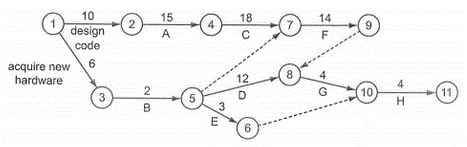
\includegraphics[width=0.7\paperwidth]{C:/Users/Admin/Desktop/Github/question_bank/LyX/static/img/9597-ALVL-2014-P2-Q1}
\par\end{center}
\begin{enumerate}
\item[(d)]  Each activity indicated by a dashed line on the PERT chart is a
dummy activity.
\begin{enumerate}
\item Explain the nature and purpose of a dummy activity.\hfill{} {[}2{]}
\item Each of the following activities matches one of the labels A-H on
the chart.
\begin{itemize}
\item write user documentation 
\item train users 
\item write code 
\item convert files
\item test code 
\item end-user testing 
\item test system 
\item install new hardware
\end{itemize}
Copy and complete the following table, 
\begin{center}
\begin{tabular}{|c|>{\centering}p{0.5\columnwidth}|}
\hline 
Label & Activity\tabularnewline
\hline 
A & \tabularnewline
\hline 
B & \tabularnewline
\hline 
C & \tabularnewline
\hline 
D & \tabularnewline
\hline 
E & \tabularnewline
\hline 
F & \tabularnewline
\hline 
G & \tabularnewline
\hline 
H & \tabularnewline
\hline 
\end{tabular}
\par\end{center}

\hfill{}{[}4{]}
\item Explain the significance of the dummy activity that leads into event
8. \hfill{}{[}3{]}
\end{enumerate}
\item[(e)]  From the PERT chart:
\begin{enumerate}
\item State the critical path.\hfill{} {[}1{]}
\item State the minimum time in which the new software can be developed
and implemented.\hfill{} {[}1{]}
\item The chart omits an activity: \textbf{write technical documentation}.
State a starting point and a finishing point for this activity. Justify
your choices. \hfill{}{[}4{]}
\end{enumerate}
\end{enumerate}
Management staff can already access the company network remotely for
other software applications. Management are to be given the facility
to access, and interact with, the customer data Via the company LAN.
However, a decision is made not to allow access to the customer data
remotely for this updated system.
\begin{enumerate}
\item[(f)]  Describe \textbf{two} methods which can be used to ensure that there
is no remote access to customer data by management staff. \hfill{}{[}4{]}
\end{enumerate}
ln the new system, customers will have access to information through
a web browser. Each customer will be able to see some information
about their purchase history.
\begin{enumerate}
\item[(g)]  Explain what software needs to be developed to provide this customer
facility. \hfill{}{[}5{]}
\item[(h)]  One of the software developers has the task of ensuring that social
issues are considered. This developer has to document these issues. 

Describe \textbf{two} issues that might be in the document with regard
to customers accessing their data. \hfill{}{[}4{]}
\end{enumerate}
{[}SPLIT\_HERE{]}
\item \textbf{{[}ALVL/9597/2019/P2/Q2{]} }

Consider the following binary tree:
\begin{center}
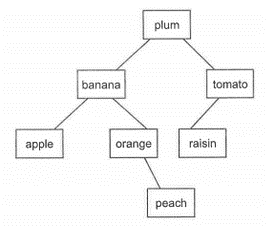
\includegraphics[width=0.35\paperwidth]{C:/Users/Admin/Desktop/Github/question_bank/LyX/static/img/9597-ALVL-2014-P2-Q2}
\par\end{center}
\begin{enumerate}
\item List the nodes, in order, that are visited for a post-order traversal.
\hfill{}{[}2{]}
\item List the nodes, in order, that are visited for an inorder traversal.
\hfill{}{[}2{]}
\item What property is exhibited by the list of items produced in \textbf{part
(b)}? \hfill{}{[}1{]}
\item Describe an algorithm, using pseudocode, to perform a binary tree
search. The output should state whether or not the item is present
in the tree. \hfill{}{[}5{]}
\end{enumerate}
{[}SPLIT\_HERE{]}
\item \textbf{{[}ALVL/9597/2019/P2/Q3{]} }

A network manager for a sales company types the following into his
computer:

\texttt{copy C:\textbackslash monthlysales\textbackslash{*}.dat
E\textbackslash :\textbackslash backup\textbackslash junesales
/V}
\begin{enumerate}
\item State the type of user interface being used. \hfill{}{[}1{]}
\item Describe, using the example, two benefits of the user interface named
in \textbf{(a)}. \hfill{}{[}4{]}
\end{enumerate}
The network manager has a disabled user who cannot use a keyboard
but can control a point-and-click device that moves a pointer on the
screen.
\begin{enumerate}
\item[(c)]  Describe a user interface that would allow this user to enter text
into a word processor. \hfill{}{[}3{]}
\item[(d)]  The sales company provides a special user interface for this user.
State\textbf{ two} benefits to the company. \hfill{}{[}2{]}
\end{enumerate}
{[}SPLIT\_HERE{]}
\item \textbf{{[}ALVL/9597/2019/P2/Q4{]} }

A small local area network (LAN) in a school consists of one switch,
one file server and ten computers.
\begin{enumerate}
\item Explain why circuit switching could be used in this LAN. \hfill{}{[}2{]}
\end{enumerate}
The network has a connection to the lnternet added.
\begin{enumerate}
\item[(b)] Explain how packet switching is used when a web page is downloaded
from the Internet. \hfill{}{[}3{]}
\end{enumerate}
A packet from the web server consists of 256 bytes. One of the bytes
is the checksum byte. In each byte one bit is the parity bit.
\begin{enumerate}
\item[(c)]  If the byte 0 0 1 1 0 1 0 1 results in a parity error, state the
type of parity being used. \hfill{}{[}1{]}
\item[(d)]  The receiving computer uses the checksum byte to check whether the
packet contains an error. Explain how it does this.\hfill{} {[}4{]}
\end{enumerate}
{[}SPLIT\_HERE{]}
\item \textbf{{[}ALVL/9597/2019/P2/Q5{]} }

A software developer is given the task of producing software for a
college. The software will help to manage information about what students
do after finishing at the college.

The destination of each student after college is classified in one
of three possible ways:
\begin{itemize}
\item University
\item Employment 
\item Other
\end{itemize}
The college wishes to store:
\begin{itemize}
\item name 
\item number of A Level passes 
\item destination (U / E / O) 
\item university attended 
\item main subject studied at university 
\item type of employment 
\item what students do when their destination is classified as 'O'
\end{itemize}
The software developer will use an objectoriented approach to developing
a solution.
\begin{enumerate}
\item Draw a class diagram which exhibits the following:
\begin{itemize}
\item suitable classes with appropriate properties and methods 
\item inheritance 
\item polymorphism \hfill{}{[}6{]}
\end{itemize}
\item Explain how your solution to (a) demonstrates software reuse.\hfill{}
{[}2{]}
\end{enumerate}
The data on the students is to be stored in a serial text file called
STUDENT.DAT. Each line of the file has the same structure:

\texttt{<Name><NoOfPasses><Destination><University><MainSubject><EmpType><Other>}

with the string NULL stored where appropriate.
\begin{enumerate}
\item[(c)]  Write an algorithm, in pseudocode, to read data from \texttt{STUDENT.DAT}
and to output the following:
\begin{itemize}
\item total number of students going to university 
\item average number of passes for the students going to university e total
number of students\hfill{} {[}7{]}
\end{itemize}
\end{enumerate}
{[}SPLIT\_HERE{]}
\item \textbf{{[}ALVL/9597/2019/P2/Q6{]} }

A function is to be written that returns the sum of all values held
in an array that are greater than a minimum value. The function will
be used with arrays of varying size, but never more than a maximum
of 50 000 elements.

A first attempt at writing the program code for the function is given
below:

\noindent %
\noindent\begin{minipage}[t]{1\columnwidth}%
\texttt{01 FUNCTION TotalSum(Results : ARRAY{[}50000{]} OF REAL, ArraySize
: INTEGER, MinValue : REAL) RETURNS REAL }

\texttt{02 \qquad{}DECLARE Sum, Counter : INTEGER }

\texttt{03 \qquad{}DECLARE Temp : Real }

\texttt{04 \qquad{}Sum = 0.0 }

\texttt{05 \qquad{}\qquad{}FOR Counter = 1 TOO ArraySize }

\texttt{06 \qquad{}\qquad{}\qquad{}Temp = Results{[}Counter{]} }

\texttt{07 \qquad{}\qquad{}\qquad{}IF Temp > MinValue THEN Sum
= Sum {*} Temp }

\texttt{08 \qquad{}\qquad{}ENDEOR }

\texttt{09 \qquad{}RETURN Sum }

\texttt{10 ENDFUNCTION}%
\end{minipage}

The function is included in a program specifically written to test
the function. The main program outputs the value returned by the function.
A compiler was used to compile the source program.
\begin{enumerate}
\item The compiler reported an error at line 5 in the function. Identify
the error and explain why it was flagged as a syntax error. \hfill{}{[}2{]}
\item The compiler also reported an error at line 8. State the type of error
reported by the compiler justifying your answer. \hfill{}{[}2{]}
\end{enumerate}
The errors indicated in \textbf{parts (a)} and \textbf{(b)} were corrected.
A successful compilation produces executable code. When the code was
executed, the program failed to complete and reports an error at line
7.
\begin{enumerate}
\item[(c)]  {} 
\begin{enumerate}
\item State the type of error that occurred. Justify your answer. \hfill{}{[}2{]}
\item The error described in \textbf{part (c) (i)} depends on the detection
of another type of error. Name this other type of error. How should
the code be changed to correct this error?\hfill{}{[}2{]}
\end{enumerate}
\end{enumerate}
When the program finally runs without error, the test plan needs to
be completed. The test plan uses data that tests different sizes of
array, different array values and different minimum values. 

The array \texttt{TempArray} is used in the main program as the array
to be processed.\quad{} 
\begin{enumerate}
\item[(d)]  Each element of \texttt{TempArray} stores a random value between
1.0 and 10.0.
\begin{enumerate}
\item Explain why the function call:

\texttt{TotalSum(TempArray, 1000, 5.0)}

is not an appropriate black box test. \hfill{}{[}2{]}
\item Explain why the function call:

\texttt{TotalSum(TempArray, 10, 10.5)}

is not an appropriate white box test. \hfill{}{[}2{]}
\end{enumerate}
\item[(e)] if each element of \texttt{TempArray} stores the value 1.0, state
a function call that will be an appropriate black box test. Justify
your answer. \hfill{}{[}3{]}
\end{enumerate}
{[}SPLIT\_HERE{]}
\end{enumerate}

\end{document}
